\section{Appendix}

\subsection{Dataset} \label{app:Dataset}

	\begin{figure}[H]
		\centering
		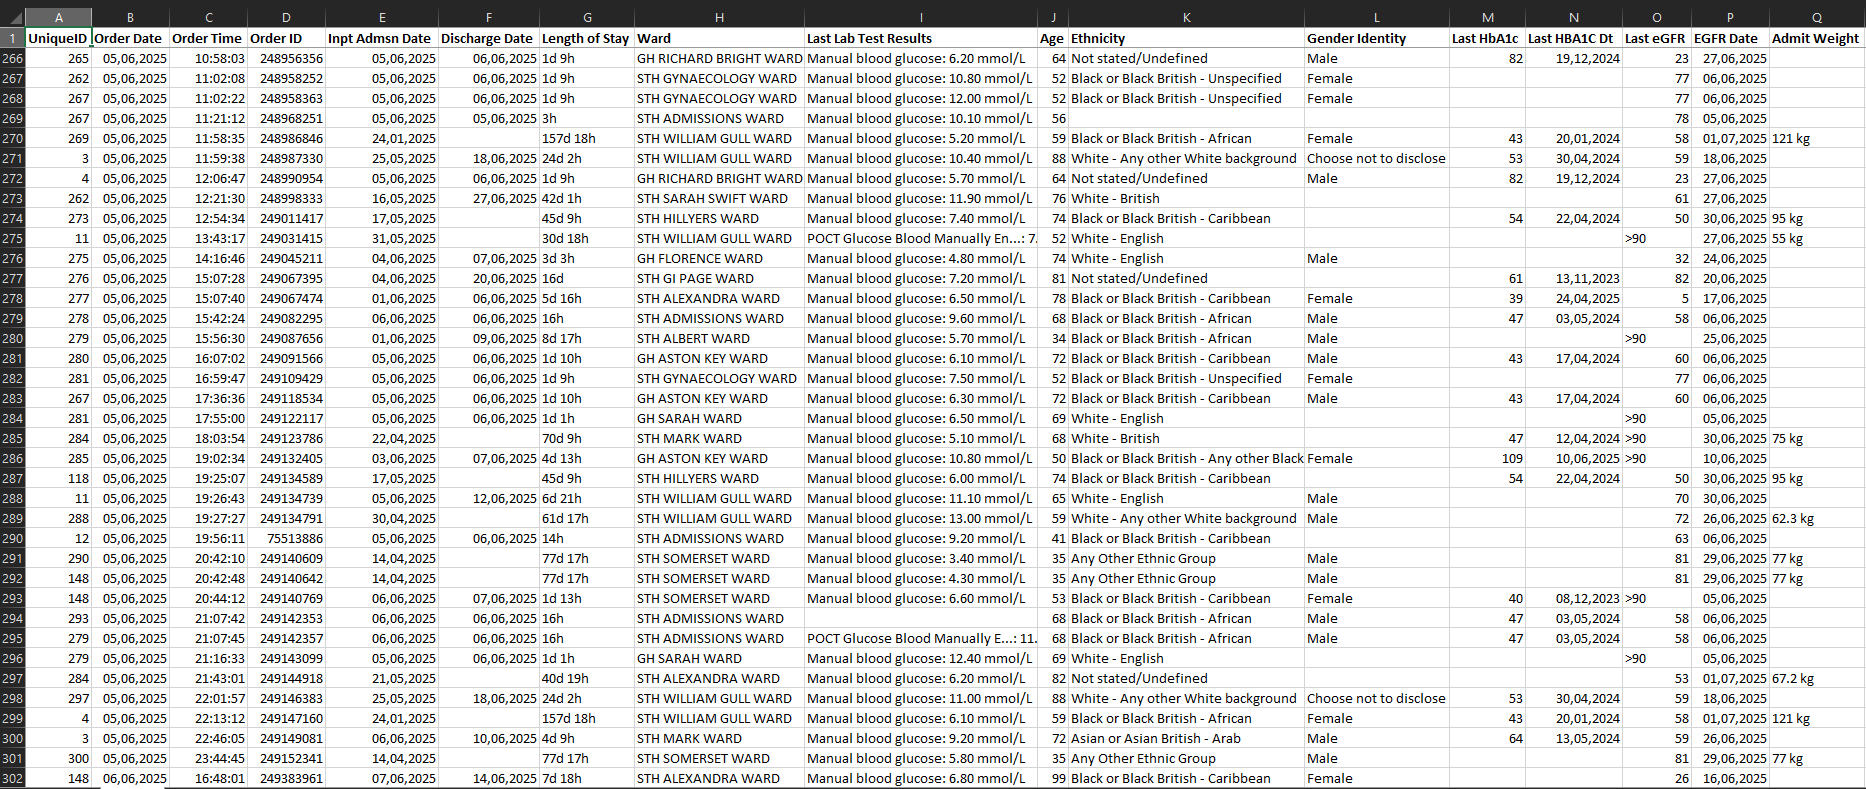
\includegraphics[width=9in, angle=90]{figures/dataset_screenshot_xl.png}
		\caption{Raw dataset}
		\label{fig:rawDataset}
	\end{figure}

	\begin{figure}[H]
		\centering
		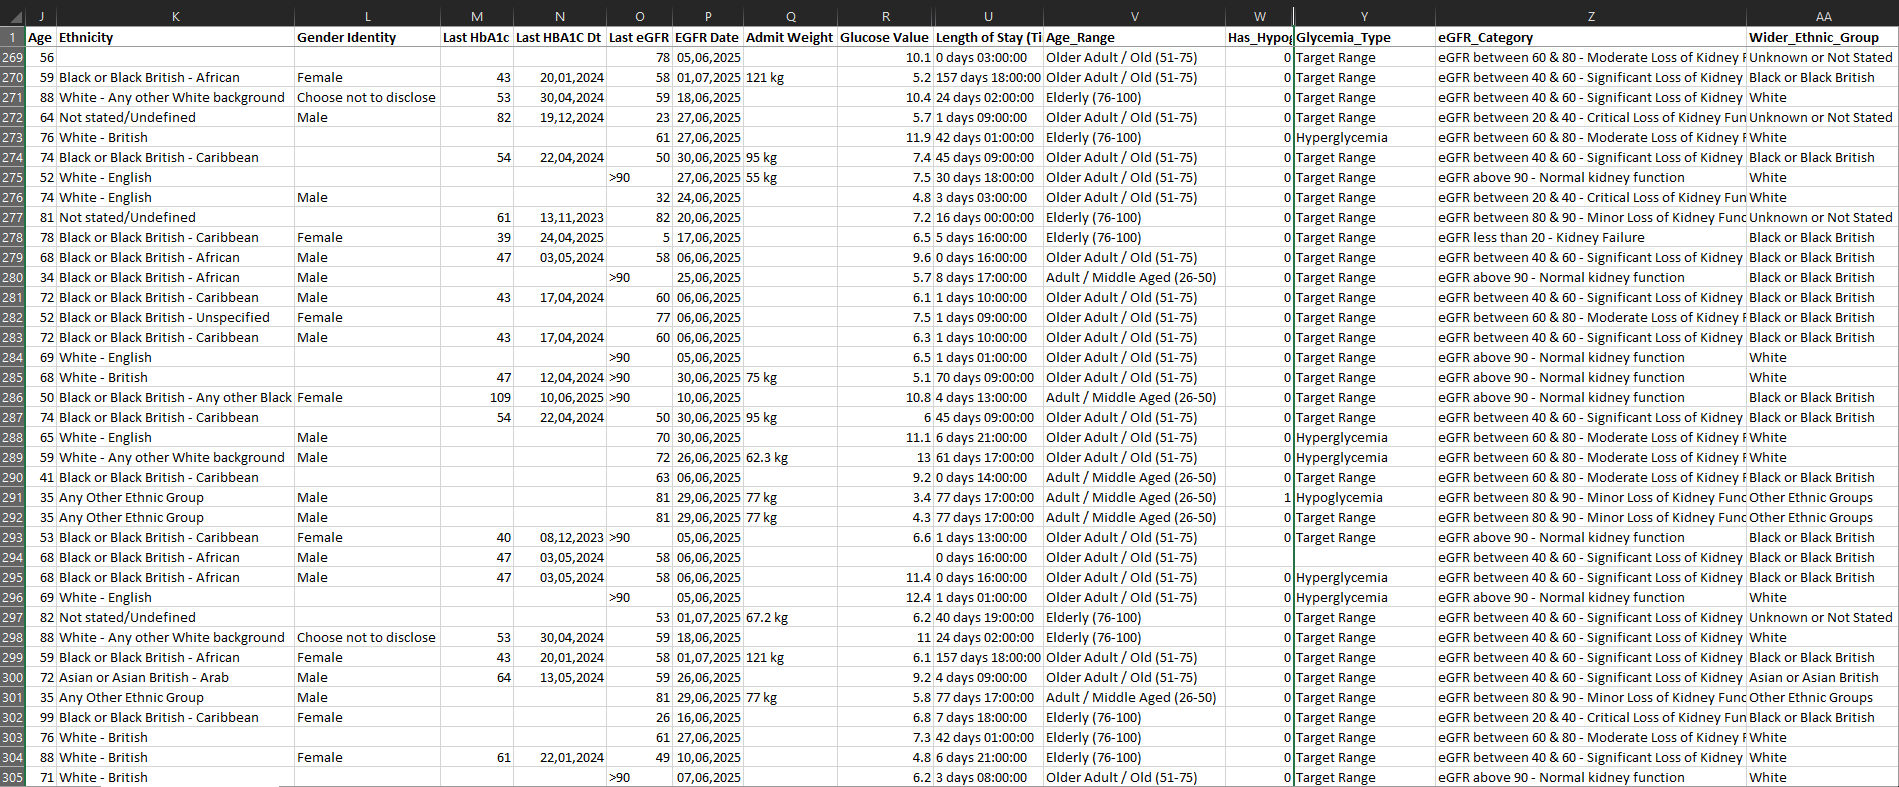
\includegraphics[width=9.5in, angle=90]{figures/cleaned_dataset_screenshot_xl.png}
		\caption{Dataset with cleaned features (this is in addition to the fields of the raw dataset)}
		\label{fig:cleanedDataset}
	\end{figure}

%  ===================================== TEMPLATE LEFTOVERS for ref ==========================================

% \red{The content of ``Appendix'' is in ``{\textbackslash}contents{\textbackslash}app\_1.tex''}

% \section{Appendix}
% 	Supplementary materials (such as source code, user menu, etc) could be included. Each appendix must be labelled (for example, Appendix A, Appendix A.1, Appendix A.2,  Appendix B, Appendix B.1, etc.) and with heading.  All Appendices must be referred in the text.  

% \subsection{Points to Note}
% Please note the following points when you write your report:
% \begin{itemize}
% 	\item Consider the outline of the report.  It is a good idea to start with the table of contents, which gives you an overall structure of the report.
% 	\item Show understanding of the topic and demonstrate the contribution of the work. 70\% of the content of the report should be your own contributions and achievements.
% 	\item Always use your own words.
% 	\item The main report and any appendices must constitute one document.
% 	\item Pages must be numbered consecutively.
% 	\item Captions must be provided for all figures and tables.
% 	\item Equations (or important equations), figures and tables must be numbered.
% 	\item All figures and tables must be referred to in the text.
% 	\item Units of all variables must be provided.
% 	\item Numerical values (floating-point number) should be in 4 decimal places.
% 	\item Contractions should not be used.
% 	\item Check the punctuation of sentences.  In particular, those sentences with equation.  For example, if an equation is at the end of a sentence, a full stop should be used.
% 	\item All variables must be defined.
% 	\item Font face of variables throughout the report (in the text, equation, figures and table) must be consistent.
% 	\item Use proper headings for chapters, sections, subsections.
% 	\item Chapters, sections, subsections should be numbered and with the same numbering system throughout the report.
% It is suggested that vector and matrix variables should be in bold, scalar variables should be in italic.
% 	\item References must be used for materials used in the report that are not yours.
% 	\item A standard reference format must be adopted and be consistently applied through the report.  General guidelines for reference format can be found on KEATS.
% 	\item Always backup your files.  
% \end{itemize}

% \section{Review of stochastic calculus}
% \subsection{Riemann integration}
% \subsection{The It\^o integral}
